\documentclass[uplatex, a4paper, 12pt, openany, oneside]{jsbook}

\usepackage[dvipdfmx]{graphicx}
\usepackage[dvipdfmx]{color}
\usepackage[dvipdfmx, bookmarks=true, setpagesize=false]{hyperref}
\usepackage{pxjahyper}

\usepackage{thesis}
\usepackage{here}
\usepackage{url}
\usepackage{subcaption}
\captionsetup[figure]{justification=centering}

\thesis{授業ノート}
\title{
  \centering
    \scalebox{1.0}{インテリジェントロボットモーション}\\
    \scalebox{0.8}{(軌道計画)}\\
    \vspace{-0.3zh}
    \scalebox{0.7}{Intelligent robot motion}\\
    \scalebox{0.7}{(Trajectory plan)}\\
    \vspace{-5.0zh}
}
\setlength{\textwidth}{\fullwidth}
\setlength{\evensidemargin}{\oddsidemargin}

\date{\today}
\vspace{-15.0zh}
\teacher{}
% \vspace{-15.0zh}
\organization{千葉工業大学 先進工学研究科 未来ロボティクス専攻}
\author{23S1022 髙橋祐樹}
\vspace{-15zh}

\renewcommand{\baselinestretch}{1.2}
\begin{document}

%% Front Matter
\frontmatter{}
%
\maketitle
%
% %!TEX root = ../thesis.tex
\chapter*{概要}
\thispagestyle{empty}
%
\begin{center}
  \scalebox{1.5}{視覚と行動のend-to-end学習により経路追従行動を}\\
  \scalebox{1.5}{オンラインで模倣する手法の提案}\\
  \scalebox{1.5}{(オフラインでデータセットを収集して訓練する手法の検証)}
\end{center}
\vspace{1.0zh}
%

近年, 自律移動ロボットの研究が盛んに行われている. 本研究室においても, 2D-LiDARを用いた自律移動システムの出力を教師信号としてロボットに与えて学習させることで, 経路追従行動をオンラインで模倣する手法を提案し, 実験によりその有効性を確認してきた. 本研究では, 従来手法を基に, 目標とする経路上及び周辺のデータを一度に収集し, オフラインで訓練する手法を提案する. 提案手法では, 経路上にロボットを配置し, カメラ画像と教師データとなる目標角速度を収集する. それらのデータを基にオフラインで学習を行い, 学習後はカメラ画像を入力とした学習器の出力により自律移動させることで, 手法の有効性を検証する. 結果として, 提案手法により経路を周回できることを確認した. 

\vspace{10mm}
キーワード: end-to-end学習, ナビゲーション, オフライン
%
\newpage
%%
\chapter*{abstract}
\thispagestyle{empty}
%
\begin{center}
  \scalebox{1.3}{A proposal for an online imitation method of path-tracking}
  \scalebox{1.3}{behavior by end-to-end learning of vision and action}
  \scalebox{1.3}{(Validation of a method to collect and train dataset offline)}
\end{center}
\vspace{1.0zh}
%

Recently, autonomous mobile robots have been studied extensively. In our laboratory, we have proposed an online imitation method of path-following behavior by training a robot with the output of a 2D-LiDAR-based autonomous mobile system as a teacher signal, and have confirmed the effectiveness of the proposed method through experiments. In this study, we propose an off-line training method based on the conventional method by collecting data on and around the target path at a time. In the proposed method, the robot is placed on the path, and camera images and target angular velocity are collected as teacher data. The effectiveness of the proposed method is verified by training the robot off-line based on these data, and after training, the robot moves autonomously by using the output of the trainer with camera images as input. As a result, it is confirmed that the proposed method is able to go around the path.

\vspace{10mm}
keywords: End-to-End Learning, Navigation, Offline 

%
\tableofcontents
%
\listoffigures
%
% \listoftables
%

%
%% Main Matter
\mainmatter{}
%
\chapter{序論}
\label{chap:introduction}
%
%\input{introduction/preface}
%
%!TEX root = ../thesis.tex

\section{はじめに}
軌道計画とは,制御対象となるシステムやロボットの動きを指定した軌道(経路)に沿って制御するための計画を立てるプロセスである.特に,バンバン制御ではオンオフの制御信号を使用して制御を行う.バンバン制御における軌道計画では,目標軌道に沿ってシステムが移動するように制御信号を生成します.制御対象が目標軌道よりも高い位置にある場合はオフ状態(制御信号がゼロ)であり,制御対象が目標軌道よりも低い位置にある場合はオン状態(最大の制御信号)となる.つまり,バンバン制御はシステムの状態が目標値を超えたり下回ったりするたびに,制御入力が急激に変化することになる. \\

次に多次元空間でのマニピュレータの軌道計画について考える.ここでの軌道とは,各自由度に対して位置,速度,及び加速度の時間履歴を指している. 

%

%
\chapter{軌道計画}
\label{chap:technology}
%
%\input{introduction/preface}
%
%!TEX root = ../thesis.tex

\section{パスの記述と計画における一般的な考慮事項 }
マニピュレータの動きはツールフレーム{T}がステーションフレーム{S}に対してどのように動くか考える.基本的な問題はマニピュレータを初期位置から最終位置まで移動させることである.つまり,ツールフレーム{T}を現在の値から望ましい最終値まで移動させたい.一般的に,この動きにはツールがステーションに対して姿勢と位置の両方が変化することが含まれる. \\

動きを詳細に指定するためには,望ましい経由点(初期位置と最終位置の間の中間点)を指定することがある.これらの経由点は,ツールがステーションに対して位置と姿勢を指定するフレームであり,初期点と最終点と共にパスポイントと呼ばれる.スムーズな動きを実現するためには,関節空間での連続性が必要であり,時間的属性も指定される場合がある.ガタガタした動きは機構の摩耗を増加させ,振動を引き起こすため,経由点間の経路には制約が必要である. \\

\section{関節空間スキーム}
ここでは,パスの生成方法を考えるが,パスの形状(空間及び時間)は関節角度の関数として記述される.通常,各パスポイントはツールフレーム{T}がステーションフレーム{S}に対して望ましい位置と姿勢で指定され,逆運動学を使用して関節角度が計算される.各関節には関係なく,滑らかな関数が見つかり,経由点での望ましい位置と姿勢が実現される.関節空間スキームは通常計算が容易であり,特異点の問題が少ないことが特徴である.  

\subsection{直方体多項式}
ツールを初期位置から目標位置に一定の時間で移動させる問題を考える.各関節には,$t_0$での値が関節の初期位置であり,$t_f$での値がその関節の望ましい目標位置である関数が必要である.\figref{Fig:fig1}に示されているように,関節の値を補間するために使用できる滑らかな関数θ(t)は多くある.スムーズな動きを行うためには,θ(t)に対して少なくとも4つの制約がある.関数に対する2つの制約は初期値と最終値の選択から来る. 

$$ θ(0)=θ_0$$
$$ θ(t_f)=θ_f \eqno(1)$$

\begin{figure}[h]
     \centering
     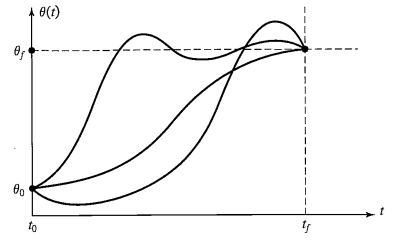
\includegraphics[keepaspectratio, scale=0.6]{images/fig1.png}
     \caption{}
     \label{Fig:fig1}
     \end{figure}

さらに2つの制約は,この関数が速度で連続であることであり,これは初期速度と最終速度がゼロであることを意味する.

$$\dot{θ}(0) = 0$$
$$\dot{θ}(t_f) = 0 \eqno(2)$$

これら4つの制約は,少なくとも3時の多項式で満たすことができる.(3時多項式は4つの係数を持つため,式(1)と(2)で与えられる4つの制約を満たすようにできる.)これらの制約によって特定の3次多項式が一意に決定される.3次多項式は次のようになる.

$$θ(t) = a_0 + a_1t + a_2t^2 + a_3t^3 \eqno(3)$$

従ってこのパスに沿った関節の速度と加速度は明確に決まる

$$\dot{θ}(t) = a_1 + 2a_2t + 3a_3t^2$$
$$\ddot{θ}(t) = 2a_2 + 6a_3t \eqno(4)$$

式(3)と(4)を4つの制約と組み合わせることで,4つの未知数に対する4つの方程式が得られる. 

$$θ_0 = a_0$$
$$θ_f = a_0 + a_1t_f + a_2t_f^2 + a_3t_f^3$$
$$0 = a_1 \eqno(5)$$
$$0 = a_1 + 2a_2t_f + 3a_3t_f^2$$

これらの方程式を解くと以下の結果が得られる. 

$$a_0 = θ_0$$
$$a_1 = 0$$
$$a_2 = \frac{3}{t_f^2}(θ_f-θ_0) \eqno(6)$$

式(6)を使用することで,任意の初期関節角度位置と望ましい最終位置を接続するための3次多項式を計算できる.この解は,関節が速度ゼロで始まり,速度ゼロで終わる場合のケースに対してのものである.
%
%
\chapter{例題}
\label{chap:old-method}
%
%\input{introduction/preface}
%
%!TEX root = ../thesis.tex

\section{EX.1}
ロータリージョイントを持つ単リンクロボットは, 初期位置であるθ = 15度で静止している. このロボットを滑らかに動かし, 3秒で目標位置であるθ = 75度に移動させたい. この動作を実現し, マニピュータを目標位置で停止させるための3次関数の係数を求める. そして, 時間の関数としてジョイントの位置, 速度, および加速度をプロットする. \\

式(6)に代入すると, 次のようになる.

$$a_0 = 15.0$$
$$a_1 = 0.0$$
$$a_2 = 20.0 \eqno(7)$$
$$a_3 = -4.44$$

式(3)と(4)を用いて, 次のように得られる.

$$θ(t) = 15.0 + 20.0t^2 -4.44t^3$$
$$\dot{θ}(t) = 40.0t - 13.33t^2 \eqno(8)$$
$$\ddot{θ}(t) = 40.0 -26.66t$$

\figref{Fig:fig2}は, この動作を40 Hzでサンプリングした際の位置, 速度, および加速度関数を示している. 任意の3次関数の速度プロファイルが放物線であり, 加速度プロファイルが直線であることに注意したい. 

\begin{figure}[h]
  \centering
  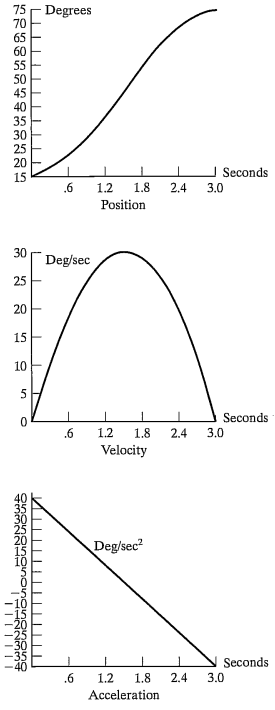
\includegraphics[keepaspectratio, scale=0.6]{images/fig2.png}
  \caption{}
  \label{Fig:fig2}
  \end{figure}
%
%
% \chapter{結言}
\label{chap:conclusion}
%
%\input{introduction/preface}
%
%!TEX root = ../thesis.tex

本研究では, 経路追従行動をカメラ画像を入力としたend-to-end学習で模倣する従来手法を基に, 目標経路上及びその周辺でデータを収集してオフラインで訓練する手法を提案した. 実験では, 経路周辺のデータを多く収集し, バッチ学習を用いて訓練を行った. これにより, テストフェーズでは成功率が100\%となり, 手法の有効性を示すことができた. また, 従来手法では訓練時間が最低でも40分必要であったのに対して, 提案手法を用いることで6分程度で訓練を終了することができた. 結果として, 訓練時間を85\%削減できることを確認した.  
%
%% Back Matter
\backmatter{}
%
\maketitle
%
% %!TEX root = ../thesis.tex
\chapter*{概要}
\thispagestyle{empty}
%
\begin{center}
  \scalebox{1.5}{視覚と行動のend-to-end学習により経路追従行動を}\\
  \scalebox{1.5}{オンラインで模倣する手法の提案}\\
  \scalebox{1.5}{(オフラインでデータセットを収集して訓練する手法の検証)}
\end{center}
\vspace{1.0zh}
%

近年, 自律移動ロボットの研究が盛んに行われている. 本研究室においても, 2D-LiDARを用いた自律移動システムの出力を教師信号としてロボットに与えて学習させることで, 経路追従行動をオンラインで模倣する手法を提案し, 実験によりその有効性を確認してきた. 本研究では, 従来手法を基に, 目標とする経路上及び周辺のデータを一度に収集し, オフラインで訓練する手法を提案する. 提案手法では, 経路上にロボットを配置し, カメラ画像と教師データとなる目標角速度を収集する. それらのデータを基にオフラインで学習を行い, 学習後はカメラ画像を入力とした学習器の出力により自律移動させることで, 手法の有効性を検証する. 結果として, 提案手法により経路を周回できることを確認した. 

\vspace{10mm}
キーワード: end-to-end学習, ナビゲーション, オフライン
%
\newpage
%%
\chapter*{abstract}
\thispagestyle{empty}
%
\begin{center}
  \scalebox{1.3}{A proposal for an online imitation method of path-tracking}
  \scalebox{1.3}{behavior by end-to-end learning of vision and action}
  \scalebox{1.3}{(Validation of a method to collect and train dataset offline)}
\end{center}
\vspace{1.0zh}
%

Recently, autonomous mobile robots have been studied extensively. In our laboratory, we have proposed an online imitation method of path-following behavior by training a robot with the output of a 2D-LiDAR-based autonomous mobile system as a teacher signal, and have confirmed the effectiveness of the proposed method through experiments. In this study, we propose an off-line training method based on the conventional method by collecting data on and around the target path at a time. In the proposed method, the robot is placed on the path, and camera images and target angular velocity are collected as teacher data. The effectiveness of the proposed method is verified by training the robot off-line based on these data, and after training, the robot moves autonomously by using the output of the trainer with camera images as input. As a result, it is confirmed that the proposed method is able to go around the path.

\vspace{10mm}
keywords: End-to-End Learning, Navigation, Offline 

%
\tableofcontents
%
\listoffigures
%
% \listoftables
%

%

\end{document}
